\section{Разработка алгоритма}
\label{sec:research:development_algotithm}

Идея, лежащая в основе всех алгоритмов сжатия с потерями, довольно проста:
\begin{itemize}
  \item на первом этапе удалить несущественную информацию;
  \item на втором этапе к оставшимся данным применить наиболее подходящий алгоритм сжатия без потерь.
\end{itemize}

Основные сложности заключаются в выделении этой несущественной информации.
Подходы здесь существенно различаются в зависимости от типа сжимаемых данных.
Для звука чаще всего удаляют частоты, которые человек просто не способен воспринять, уменьшают частоту дискретизации,
а также некоторые алгоритмы удаляют тихие звуки, следующие сразу за громкими, для видеоданных кодируют только движущиеся объекты,
а незначительные изменения на неподвижных объектах просто отбрасывают. Для одиночных изображений, как и для звука,
отсеиваются элементы которые человек не способен различить.
Методы выделения несущественной информации на изображениях будут подробно рассмотрены далее.

\subsection{Критерии качества сжатого изображения}
\label{sub:research:errors}

Прежде чем говорить об алгоритмах сжатиях с потерями, необходимо договориться о том,
что считать приемлемыми потерями. Понятно, что главным критерием остаётся визуальная оценка изображения,
но также изменения в сжатом изображении могут быть оценены количественно.
Самый простой способ оценки --- это вычисление непосредственной разности сжатого и исходного изображений.

\begin{equation}
  \label{eq:research:image_delta}
  error = \sum_{i=1}^{N}\sum_{j=1}^{M}\left | s_{i,j}-a_{i,j} \right |
\end{equation}
\begin{explanation}
где & $ s_{i,j} $ & значение пикселя в позиции i,j исходного изображения;\\
  & $ a_{i,j} $ & значение пикселя в позиции i,j сжатого изображения изображения;\\
  & $ N $ & высота изображения в пикселях;\\
  & $ M $ & ширина изображения в пикселях.
\end{explanation}

Очевидно, что, чем больше суммарная ошибка, тем сильнее искажения на сжатом изображении.
Тем не менее, эту величину крайне редко используют на практике, т.к. она никак не учитывает размеры изображения,
а значит не поможет оценить метод сжатия изображений разной величины.
Гораздо шире применяется оценка с использованием среднеквадратичного отклонения~\cite{quadratic_deviation}:

\begin{equation}
  \label{eq:research:image_standard_deviation}
  error = \sqrt{\frac{\sum_{i=1}^{N}\sum_{j=1}^{M}(s_{i,j}-a_{i,j})^{2}}{N*M}}
\end{equation}
\begin{explanation}
где & $ s_{i,j} $ & значение пикселя в позиции i,j исходного изображения;\\
  & $ a_{i,j} $ & значение пикселя в позиции i,j сжатого изображения изображения;\\
  & $ N $ & высота изображения в пикселях;\\
  & $ M $ & ширина изображения в пикселях.
\end{explanation}

Другой подход заключается в следующем: пиксели итогового изображения рассматриваются как сумма пикселей исходного изображения и шума.
Критерием качества при таком подходе называют величину отношения сигнал-шум (SNR), вычисляемую следующим образом:

\begin{equation}
  \label{eq:research:image_snr}
  SNR = \sqrt{\frac{\sum_{i=1}^{N}\sum_{j=1}^{M}a_{i,j}^{2}}{\sum_{i=1}^{N}\sum_{j=1}^{M}(s_{i,j}-a_{i,j})^{2}}}
\end{equation}
\begin{explanation}
где & $ s_{i,j} $ & значение пикселя в позиции i,j исходного изображения;\\
  & $ a_{i,j} $ & значение пикселя в позиции i,j сжатого изображения изображения;\\
  & $ N $ & высота изображения в пикселях;\\
  & $ M $ & ширина изображения в пикселях.
\end{explanation}

Две последние формулы будут использоваться для оценки качества полученного изображения.

\subsection{Выбор нейронной сети}
\label{sub:research:neuro}

В отличие от традиционных методов сжатия --- математического вычисления и удаления избыточности --- нейронная сеть при
решении задачи сжатия исходит из соображений нехватки ресурсов. Топология сети и ее алгоритм обучения таковы,
что данные большой размерности требуется передать со входа нейронной сети на ее выходы через сравнительно небольших размеров канал.
Для реализации сжатия такого рода может использоваться многослойный перцептрон следующей архитектуры:
\begin{itemize}
  \item количество нейронов во входном и выходном слое одинаково и равно размерности сжимаемых данных;
  \item между этими слоями располагаются один или более промежуточных слоев меньшего размера.
\end{itemize}
Число промежуточных слоев определяет степень сложности преобразования данных. Например сеть с тремя промежуточными слоями
может выполнять лучшее сжатие на обучающих данных, но может дать худший результат в реальных ситуациях. Это связано с тем,
что в исходных данных может случайно образоваться некая зависимость, которая не имеет никакого отношения к реальности.
Исходные данные для сети составляются таким образом, чтобы на выходах был всегда тот же набор сигналов, что и на входе.
В процессе работы алгоритм обратного распространения ошибки минимизирует ошибку. Это означает, что веса связей от входного слоя нейронов и,
примерно, до серединного слоя будут работать на компрессию сигнала, а остальные --- на его декомпрессию.
При практическом использовании полученную сеть разбивают на две. Вывод первой сети передают по каналу связи и подают на вход второй,
которая осуществляет декомпрессию(рисунок~\ref{fig:bottleneck_achitecture}).

\begin{figure}[ht]
\centering
  \includegraphics[scale=0.5]{neural_network_bottleneck_achitecture.jpg}
  \caption{ «Бутылочное горлышко» — одна из возможных топологий нейросетей. }
  \label{fig:bottleneck_achitecture}
\end{figure}

\subsection{Построение схемы алгоритма}
\label{sub:research:algorithm}

Для построения прототипа необходимо сформировать последовательность операций на исходным изображением.
Распишем этапы сжатия последовательно:
\begin{itemize}
  \item загрузка матрицы пикселей;
  \item преобразование значений пикселей в сигналы для нейронной сети;
  \item разбиение матрицы сигналов на блоки;
  \item выбор соотношения количества входных нейронов к количеству нейроннов в срединном слое;
  \item выбор необходимого количества блоков для обучения сети;
  \item обучение нейронный сети на выбранных блоках;
  \item разделение сети на кодер и декодер;
  \item кодирование изображение при помощи кодера;
  \item сохранение декодера и полученных данных;
  \item сжатие методом без потерь сохраненных данных;
\end{itemize}

Загрузка изображений будет производится в двухмерный массив, где каждому пикселю исходного изображения будет соответствовать
число от 0 до 255. На данном этапе будем сжимать только черно-белые изображения.

Далее нам необходимо преобразовать исходную матрицу в матрицу сигналов. Сигнал --- это вещественное число от -1 до 1.
\begin{equation}
  \label{eq:research:image_to_signals}
  signal = (pixel + 1)/128-1
\end{equation}
\begin{explanation}
где & $ pixel $ & значение пикселя, лежащее в диапазоне 0..255.
\end{explanation}

Следующий этап --- разбиени матрицы сигналов на блоки.
Размер блока будет влиять на размер нейронной сети и соответственно на скорость ее обучения.
В реализации алгоритма попробуем использовать блоки разного размера.

На этапе выбора соотношения количества входных нейронов к количеству нейроннов в срединном слое,
фактически идет выбор степени сжатия изображения. Если количество входных нейроннов будет 2 раза больше,
чем количество нейроннов в срединном слое, то данные сожмуться в 2 раза.

На этапе подготовки выборки, следует учитывать несколько моментов:
\begin{itemize}
  \item большое количество тестов ведет к повышению качества изображения;
  \item большое количесво тестов замедляет обучение сети, а соответственно замедляет процесс сжатия;
  \item тестовые данные должны удолетворять критериям репрезентативности и непротиворечивости.
\end{itemize}

Обучение сети будет производидится алгоритмом обратного распространения ошибки. На каждой итерации алгоритма обратного распространения
весовые коэффициенты нейронной сети модифицируются так, чтобы улучшить решение одного примера. Следовательно будем применять алгоритм к
каждому выбранному блоку на предыдущем этапе, пока не достигнем необходимой точности(разницы между входным и выходными сигналами).

Следующий этап --- разделение нейронной сети на кодер и декодер. Это необходимо для того, чтобы кодером сжать исходные сигнялы в новую матрицу сигналов.
Декодер вместе с новой матрицей сигналов сохраняется с применением метода сжатия без потерь.

Этапы открытия изображения для просмотра:
\begin{itemize}
  \item загрузить сохраненный данные;
  \item декодировать сжатые данные;
  \item из полученных данных выделить декодер и матрицу сигналов;
  \item с помощью декодера преобразовать матрицу сигналов;
  \item выполнить обратное преобразование матрицы сигналов в матрицу пикселей.
\end{itemize}

В результате мы получили алгоритм преобразования изображения для сжатия и сохранения,
а так же алгоритм для открытия сжатого изображения. Реализация данных алгоритмов будет описана в следующей главе.
